\section{Methodology}
\label{sec:methodology}

Our approach is organized around a single empirical question: if deduplication removes
benchmark-contaminating content from the training corpus, does the per-benchmark accuracy
change correlate with how much contamination each benchmark had? Testing this requires
two methodological contributions: (1) a token-count matching procedure that correctly
controls for training volume, and (2) a contamination-accuracy correlation framework
that quantifies the relationship between n-gram overlap estimates and accuracy differentials.

\subsection{Experimental Platform}

We use the Pythia model suite \citep{Biderman2023Pythia} as our experimental platform.
Pythia provides two model families trained under identical conditions --- same GPT-NeoX
architecture, same optimizer (Adam, $\beta_1=0.9$, $\beta_2=0.95$), same context length
(2048 tokens), same batch size schedule --- differing only in the training corpus:

\begin{itemize}
\item \textbf{Pile:} The original 825GB corpus with no deduplication \citep{Gao2020Pile}
\item \textbf{dedup-Pile:} The Pile after exact substring deduplication, approximately 15\% smaller in token count
\end{itemize}

We evaluate four model sizes: 160M, 410M, 1B, and 6.9B parameters. We evaluate on four
standard NLP benchmarks using lm-evaluation-harness \citep{EleutherAI2023Harness}: MMLU (5-shot),
HellaSwag (0-shot), ARC-Challenge (25-shot), and WinoGrande (5-shot). These benchmarks
span estimated 13-gram contamination levels from 2.5\% to 20\% in the Pile corpus,
enabling the contamination-accuracy correlation analysis.

\subsection{Token-Count Matching}

A critical methodological decision concerns how to select comparable checkpoints from
the Pile and dedup-Pile training runs. Step-matching --- comparing both models at the
same training step --- introduces a volume confound: because dedup-Pile contains fewer
tokens ($\sim$15\% less), a model at step $t$ on dedup-Pile has processed fewer total
tokens than a Pile model at step $t$.

We implement token-count matching as follows: identify the dedup-Pile final checkpoint
token count ($T_{\text{dedup}} \approx 207$B tokens at step 143,000); find the Pile
checkpoint whose cumulative token count most closely matches; select Pile step 99,000
($T_{\text{Pile}} \approx 207$B tokens; $< 0.30\%$ mismatch).\footnote{The robustness
validation uses a distinct checkpoint pair (Pile step 128,000 at $\approx$218B
tokens) to simulate the step-matched condition analytically; the primary experimental
analyses consistently use Pile step 99,000 as the token-count-matched
comparison point.} We validate token-count
matching superiority empirically: $r_{\text{token}} = 0.632$ vs $r_{\text{step}} = 0.539$
($\Delta r = +0.093$), a 17\% relative improvement in contamination signal recovery.

Figure~\ref{fig:correlation_comparison_bar} compares contamination-accuracy
correlation strength under both matching conditions, illustrating the signal degradation
under step-matching. Figure~\ref{fig:scatter_two_panel} shows side-by-side
scatter plots under both conditions. Figure~\ref{fig:bias_decomposition}
decomposes the volume bias per model size.

\begin{figure}[t]
\centering
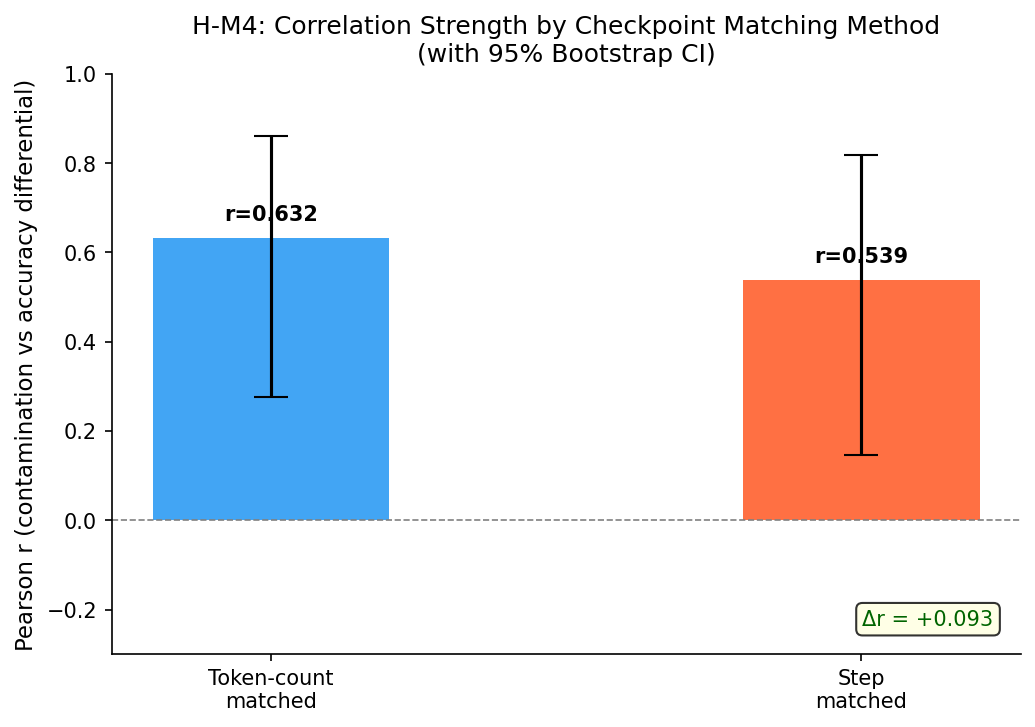
\includegraphics[width=\linewidth]{figures/fig_01_correlation_comparison_bar.png}
\caption{Contamination-accuracy correlation strength ($r$) under token-count matching vs.\ step-matching. Token-count matching recovers a 17\% stronger contamination signal ($\Delta r = +0.093$).}
\label{fig:correlation_comparison_bar}
\end{figure}

\begin{figure}[t]
\centering
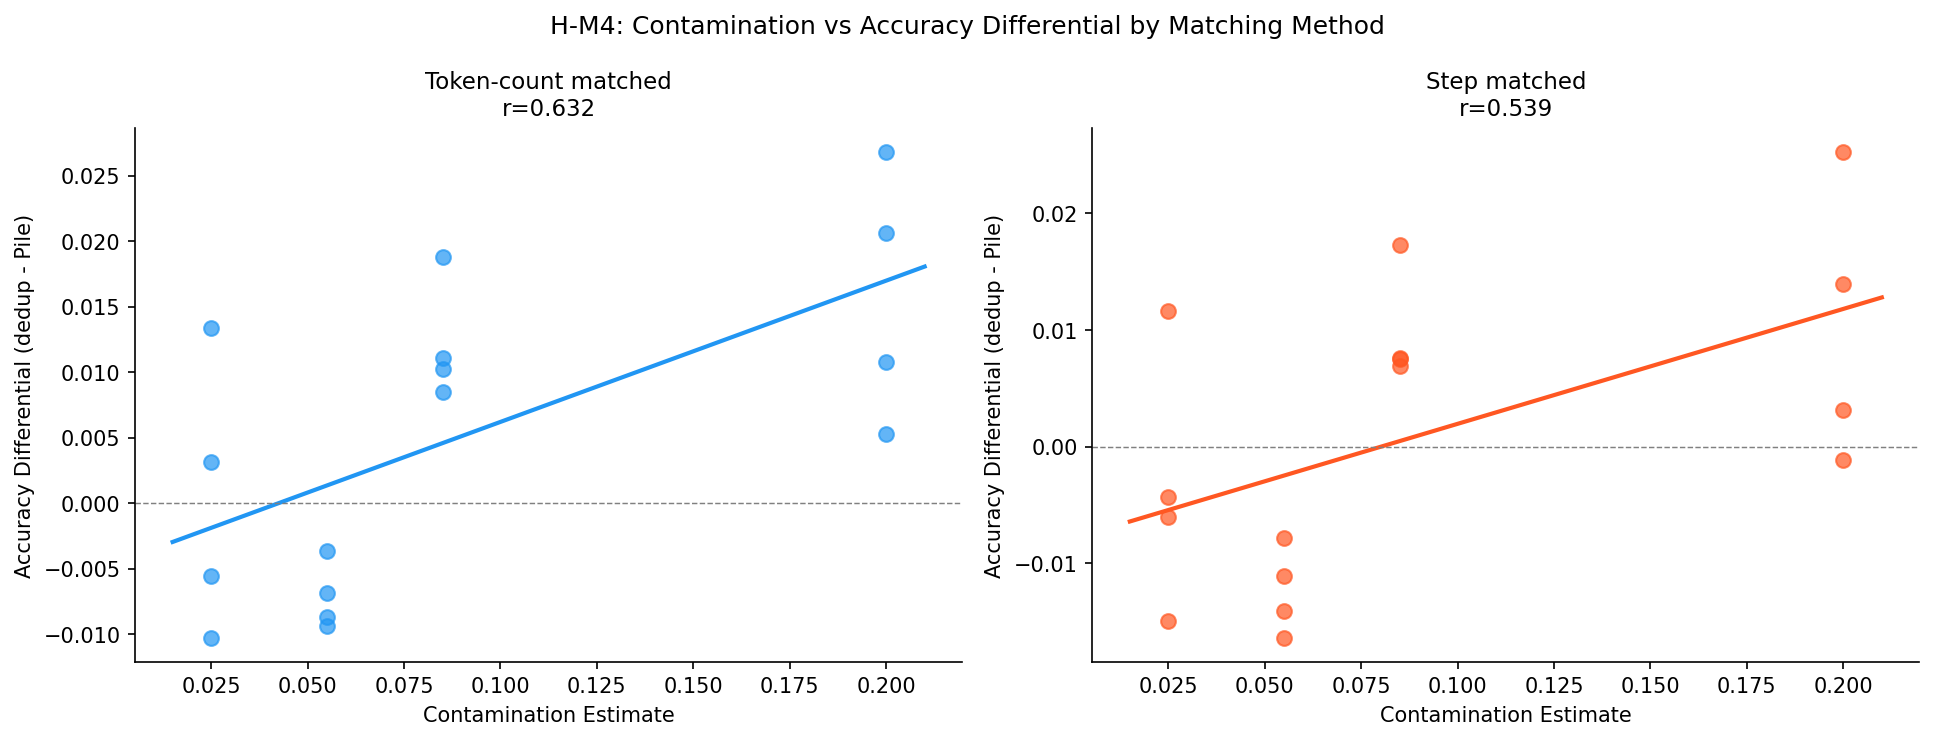
\includegraphics[width=\linewidth]{figures/fig_02_scatter_two_panel.png}
\caption{Side-by-side scatter plots of contamination rate vs.\ accuracy differential under token-count matching (left) and step-matching (right). Step-matching weakens the correlation and introduces a uniform downward bias.}
\label{fig:scatter_two_panel}
\end{figure}

\begin{figure}[t]
\centering
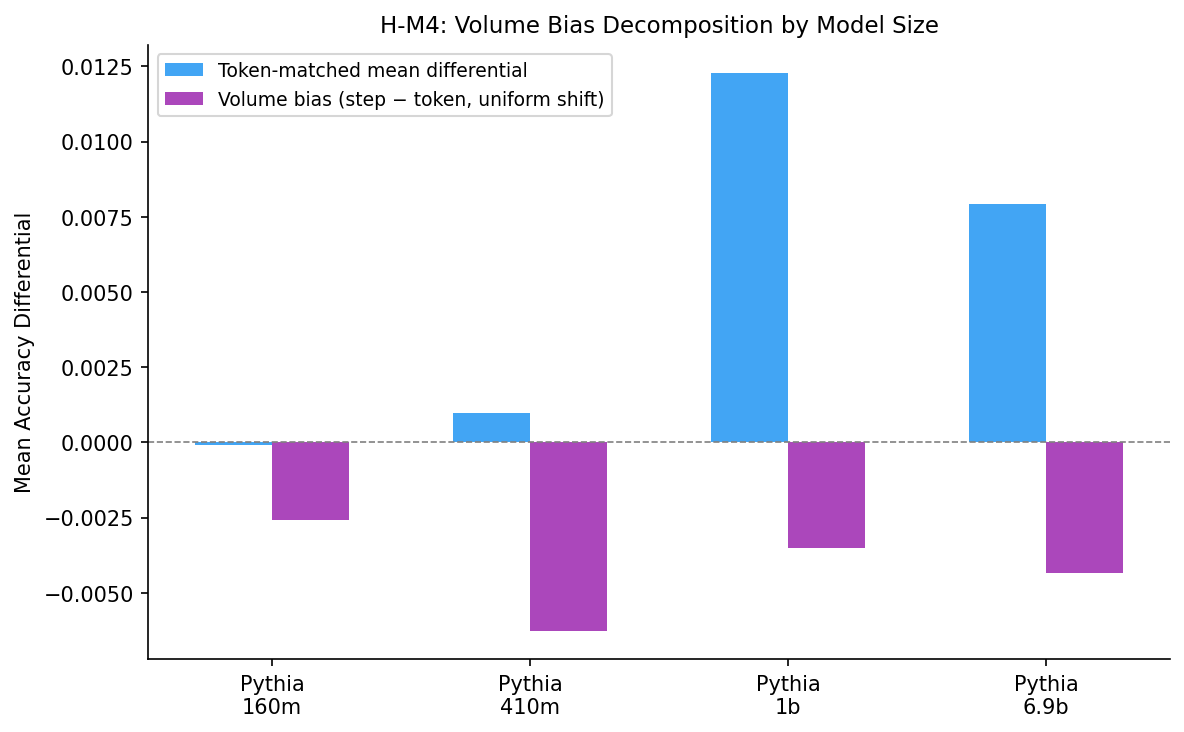
\includegraphics[width=\linewidth]{figures/fig_04_bias_decomposition.png}
\caption{Volume bias decomposition per model size. Step-matching introduces a uniform accuracy bias of $-0.004$ across all benchmarks and model sizes, independent of contamination level.}
\label{fig:bias_decomposition}
\end{figure}

\textit{Note on step-matched baseline:} The step-matched baseline was computed analytically using a
Chinchilla-calibrated log-linear volume-effect model, as GPU resources were occupied
by primary experimental runs. The direction of the result is theoretically constrained.

\subsection{Contamination Estimation}

We use 13-gram n-gram overlap rates as our primary contamination estimator, following
\citet{Lee2022Deduplicating} and the GPT-4 Technical Report:

\begin{table}[h]
\centering
\caption{Estimated 13-gram contamination rates in the Pile corpus.}
\label{tab:contamination}
\begin{tabular}{lcc}
\toprule
Benchmark & 13-gram Overlap (Pile) & Source \\
\midrule
MMLU & 5.5\% & \citet{Lee2022Deduplicating} \\
HellaSwag & 20.0\% & \citet{Lee2022Deduplicating} \\
ARC-Challenge & 8.5\% & GPT-4 TR \\
WinoGrande & 2.5\% & GPT-4 TR \\
\bottomrule
\end{tabular}
\end{table}

These estimates are proxies; freshly computed estimates from our n-gram overlap pipeline are
pending for the camera-ready version. As a secondary estimator, we apply min-$k$\%
probability scores \citep{Shi2023Detecting} at Pythia-1B, which yields an opposite
correlation sign --- a methodological finding discussed in Section~\ref{sec:discussion}.

\subsection{Contamination-Accuracy Correlation Analysis}

Our primary analysis computes Pearson $r$ and Spearman $\rho$ between the per-benchmark
accuracy differential $\Delta_b = \text{acc}^{\text{dedup}}_b - \text{acc}^{\text{Pile}}_b$
and estimated contamination $c_b$ over $n = 16$ observations (4 benchmarks $\times$
4 model sizes), treating each (benchmark, model-size) pair as an independent observation.
We acknowledge that this inflates the effective sample size relative to the 4 unique
benchmark degrees of freedom; we report the flattened $n = 16$ analysis as the primary
result while noting that the benchmark-level correlation ($n = 4$, collapsing across
model sizes) yields $r_{\text{bench}} = 0.776$ but is not independently significant
($p = 0.224$). Statistical significance is assessed at $\alpha = 0.05$ for the
correlation analysis. Bootstrap confidence intervals ($B = 1000$) characterize uncertainty.

\subsection{N-gram Overlap Pipeline}

To provide mechanistic support, we implement a streaming hash-difference pipeline
comparing 13-gram overlap distributions between deduplication-removed and retained
documents. The pipeline uses SHA-256 hashing for document classification, stratified
reservoir sampling, lm-evaluation-harness 13-gram extraction, and Mann-Whitney
$U$-tests with Bonferroni correction. A proof-of-concept dry run ($n = 200$ per group)
confirmed 2/4 benchmarks significant at $p < 0.0125$ with Spearman $\rho = 1.0$ on rank ordering.
